\chapter{Introduction}
\label{chapter:introduction}

\newthought{The introduction chapter} begins here, starting with small caps like Tufte does, using the \verb|\newthought| command (which you can also use to start a new thought within a section. This style is based on Edward Tufte's (TOUGH-tee) books.\cite{Tufte2001,Tufte1990,Tufte1997,Tufte2006} There are many cheats and shortcuts to approximate Tufte's style, like using Palatino, Helvetica, and Bera Mono rather than Tufte's actual fonts like Bembo and Gill Sans. More detail about what styles to use within this class, see \href{https://ctan.org/pkg/tufte-latex}{Tufte Latex}.

\section{Floats}\label{sec:overview}

\newthought{Each section} also starts with small caps. Okay, you probably noticed the huge margins. You don't necessarily have to use them all the time. For example, I could cite Tufte here~\citep{Tufte2001} by using the \verb|\citep| instead of the \verb|\cite| command, which makes marginal citations.

\subsection{Subsection}

By the way, there are subsections, but no sub-subsections. This is on purpose.

\begin{marginfigure}%
  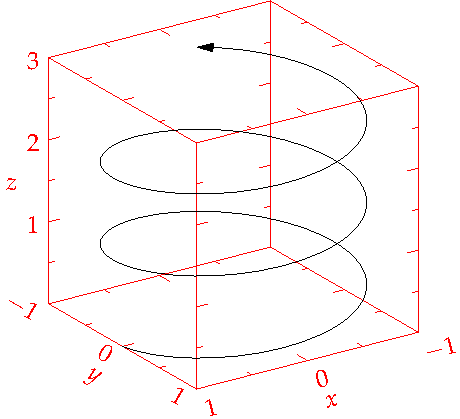
\includegraphics[width=\linewidth]{introduction/helix}
  \caption{This is a margin figure.  The helix is defined by 
    $x = \cos(2\pi z)$, $y = \sin(2\pi z)$, and $z = [0, 2.7]$.  The figure was
    drawn using Asymptote (\url{http://asymptote.sf.net/}).}
  \label{fig:marginfig}
\end{marginfigure}

\paragraph{Paragraph} 

The paragraph command is as small as it gets.

\subsection{Floats again}

Anyway, part of the reason to use this class is the use of sidenotes\sidenote{Like this one, introduced with \texttt{sidenote} or \texttt{footnote}.} and margin notes. Margin notes work the same but have no superscript to refer back to the text.

You can also put figures and tables in the margins using the \texttt{marginfigure} and \texttt{margintable} environments, and reference them as normal, like Fig.~\ref{fig:marginfig}. A trick with these is that they sometimes run into each other, in which case you should use the optional offset like \verb|\begin{margintable}[-5em]|. Similar options exist for sidenotes and margin notes, so checkout \href{https://ctan.org/pkg/tufte-latex}{Tufte LaTeX} for more info. Sidenotes are also great for short code listings.\footnote{\vspace{-1em}\begin{lstlisting}^^J
glm(y ~ m * x + b, 
    family = "binomial")^^J
\end{lstlisting}
}

Anyway, of course not everything can go in the margin, and for that we have the \texttt{figure} and \texttt{figure*} environment, for normal text width and full page width, respectively.
\begin{figure*}[h]
  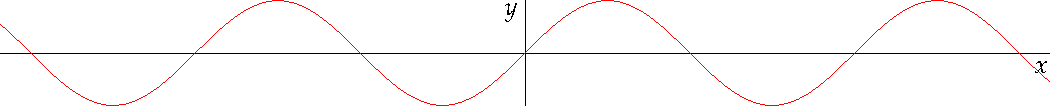
\includegraphics[width=\linewidth]{introduction/sine.pdf}%
  \caption{This graph shows $y = \sin x$ from about $x = [-10, 10]$.
  \emph{Notice that this figure takes up the full page width.}}%
  \label{fig:fullfig}%
\end{figure*}

\begin{figure}
  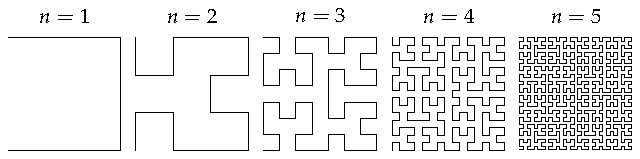
\includegraphics{introduction/hilbertcurves.pdf}
%  \checkparity This is an \pageparity\ page.%
  \caption[Hilbert curves of various degrees $n$.][6pt]{Hilbert curves of various degrees $n$. \emph{Notice that this figure only takes up the main textblock width.}}
  \label{fig:textfig}
  %\zsavepos{pos:textfig}
\end{figure}

\section{By the way}

Please use \texttt{booktabs}-style tables, please. Please. They look like Table~\ref{tab:example}.

\begin{table}[h]
\centering
\begin{tabular}{l l l l}
\toprule
\textit{Name}	& \textit{Species}	& \textit{Age}	& \textit{Smell}	\\
\midrule
Phillipe		& Otter				& 5			& musky					\\ \rowcolor{lightgray}
T\'{e}odor		& Bear				& $\sim$35	& bachelor-esque		\\
Molly			& Cat				& $>$100	& fresh laundry			\\ \rowcolor{lightgray}
Liebot			& Robot				& ???		& Drakkar Noir			\\
\bottomrule
\end{tabular}
\caption{The way that tables should look.}
\label{tab:example}
\end{table}

\vspace{1em}
The zebra-striping (achieved using \verb|\rowcolor|) and title italics are optional, but the point is not to have a thousand thick black lines obscuring the information. Analogous to figures, variants \texttt{margintable}, \texttt{table}, and \texttt{table*} exist. Please just don't use them to make tables like \ref{tab:ugly}.
\begin{margintable}
\centering
\begin{tabular}{|l|l|l|}
\hline
\textbf{Alg}	& \textbf{P}		& \textbf{AUC}		\\ \hline\hline
BF-1000	& \textbf{$\mathbf{0.67}$**}	& \textbf{$\mathbf{0.81}$**}	\\ \hline
MTG-MN	& $0.54$			& $0.32$			\\ \hline
RM-DL2	& $0.33$			& $0.48$			\\ \hline
3CPO	& $0.45$			& $0.22$			\\ \hline
\end{tabular}
\caption{A distractingly ugly and overwrought margin table with obscure abbreviations.}
\label{tab:ugly}
\end{margintable}

\section{Speaking of which}

If you want it all to go together nicely, I suggest making figures in R. My favorite practical guide to making Tufte-like graphs is \href{http://motioninsocial.com/tufte/}{Tufte in R} by Lukasz Piwek.